\documentclass[answers]{exam} 
%\documentclass{exam} 
\usepackage{amsmath,amssymb,comment,enumitem,
%fdsymbol,
float,tikz,pgfplots,etoolbox,ifthen,mdframed,fullpage,graphicx,environ,xcolor,array,float} 
\usepackage{listings}
\usepackage{tabularray}
\usepackage{booktabs}
\usepackage{amsthm}

\usepackage[hyperfootnotes=false,hidelinks]{hyperref}
\pgfplotsset{compat=1.17}

\mdfdefinestyle{QuoteFrame}{% Tweak the following to taste
    linecolor=blue,
    outerlinewidth=2pt,
    roundcorner=40pt,
    innertopmargin=\baselineskip,
    innerbottommargin=\baselineskip,
    innerrightmargin=20pt,
    innerleftmargin=20pt, 
    backgroundcolor=gray!20!white}
    
%%%%%%%%%%%%%%%%%%%%%%%%%%%%%%%%%%%%%%%%%%%%%%%%%%%%%%%%%%%%%%%
% Add some star options
%%%%%%%%%%%%%%%%%%%%%%%%%%%%%%%%%%%%%%%%%%%%%%%%%%%%%%%%%%%%%%%
\usetikzlibrary{shapes.geometric, calc} %testing stars...  use \starscore{numStarsFilled}{numStarsTotal} -kmp
\newcommand\starscore[2]{%
  \pgfmathsetmacro\pgfxa{#1 + 1}%
  \tikzstyle{scorestars}=[star, star points=5, star point ratio=2.5, draw, inner sep=0.12em, anchor=outer point 3]%
  \begin{tikzpicture}[baseline=2pt]
    \foreach \i in {1, ..., #2} {
      \pgfmathparse{\i<=#1 ? "black" : "white"}
      \edef\starcolor{\pgfmathresult}
      \draw (\i*1em, 0) node[name=star\i, scorestars, fill=\starcolor, semithick]  {};
    }
    \pgfmathparse{#1>int(#1) ? int(#1+1) : 0}
    \let\partstar=\pgfmathresult
    \ifnum\partstar>0
      \pgfmathsetmacro\starpart{#1-(int(#1)}
      \path [clip] ($(star\partstar.outer point 3)!(star\partstar.outer point 2)!(star\partstar.outer point 4)$) rectangle 
      ($(star\partstar.outer point 2 |- star\partstar.outer point 1)!\starpart!(star\partstar.outer point 1 -| star\partstar.outer point 5)$);
      \fill (\partstar*1em, 0) node[scorestars, fill=black]  {};
    \fi
  \end{tikzpicture}%
}

% \renewcommand\starscore[2]{\relax}   % Disable \starscore for testing

\usepackage[normalem]{ulem}
\addpoints
\marksnotpoints

\definecolor{MyGreen}{rgb}{0.1, 0.4, 0.1}
\definecolor{MyBlue}{rgb}{0.1, 0.1, 0.9}

\AtBeginEnvironment{solution}{\color{MyGreen}}

\newboolean{NoSolutions} 
% Select one of the following two active lines.
% (The \setboolean command allows you to use ifthen)
%\noprintanswers\setboolean{NoSolutions}{true}
\printanswers  \setboolean{NoSolutions}{false}

%Add rubrics
\usepackage{tagging}
% Comment out this line to hide the rubric text:
\usetag{rubric}

\newcommand\pts[1][2]{\textcolor{MyBlue}{\text{\bf [#1 pts]}}}
\newcommand\pt{\textcolor{MyBlue}{\text{\bf [1 pt]}}}

\newcommand\rubric[1]{\tagged{rubric}{\textcolor{MyBlue}{#1}}}

\newenvironment{rubricEnv}{\taggedblock{rubric} \color{MyBlue}}{\endtaggedblock}

\newcommand{\onestar}{\raisebox{0.05cm}{\resizebox{1.6cm}{!}{$\bigstar\largewhitestar\largewhitestar\largewhitestar$ \ }}}
\newcommand{\twostar}{\raisebox{0.05cm}{\resizebox{1.6cm}{!}{$\bigstar\bigstar\largewhitestar\largewhitestar$ \ }}}
\newcommand{\threestar}{\raisebox{0.05cm}{\resizebox{1.6cm}{!}{$\bigstar\bigstar\bigstar\largewhitestar$ \ }}}
\newcommand{\fourstar}{\raisebox{0.05cm}{\resizebox{1.6cm}{!}{$\bigstar\bigstar\bigstar\bigstar$ \ }}}

\usepackage{mathrsfs}
\newcommand{\Laplace}{\mathscr{L}}

\newcommand{\lr}[3]{\left#1{\mathstrut#3}\right#2}
\newcommand{\abs}[1]{\lr\vert\vert{#1}}
\renewcommand{\half}{\frac{\textstyle 1}{\textstyle 2}}
\renewcommand{\o}{\omega}
\renewcommand{\a}{\alpha}
\renewcommand{\b}{\beta}
\renewcommand{\bar}[1]{\mskip.5\thinmuskip\overline{\mskip-.5\thinmuskip {#1} \mskip-.5\thinmuskip}\mskip.5\thinmuskip}
\newcommand{\wt}{\widetilde}
\newcommand{\wh}{\widehat}
\newcommand{\Set}[1]{\lr\lbrace\rbrace{#1}}

\everymath{\displaystyle}
\newcommand{\diff}[2]{\frac{\text{d}#1}{\text{d}#2}}


\begin{document}

\subsection*{MATH 101A --- ASSIGNMENT 4}

\subsubsection*{Learning goals}
\begin{itemize}
    \setlength\itemsep{0.1em}
    \item Consolidate ideas of convergence and numerical approximation for series.
    \item Use Fourier methods to find some exact sums.
    \item Apply concepts from geometric series in support of larger problems.
    \item Be amazed by the ingenuity and power of Feymann's Integral Trick.
\end{itemize}

\subsubsection*{Contributors}

\textit{On the first page of your submission, list the student numbers and full names (with the last name in \textbf{bold}) of all team members. Indicate members who have not contributed using the comment ``(non-contributing)''.}

\begin{itemize}
    \item \#00000000 Randy {\bf Zhu}
\end{itemize}

\subsubsection*{Reflection question}

\textit{Reflection questions encourage you to think about how mathematics is done. This is an important ingredient of success. Reflection questions contribute to your \textbf{engagement grade}.}

\begin{questions}

\question Each member of your team should submit an individual response for part (a). Part (b) may be done as a group or individually. Part (c) should be done as a group. You will not be evaluated on what you write here; use this question as a prompt for your own honest review, reflection, and preparation.

\begin{parts}
\part (individual) Review your preparation and your performance on Test 1 and Test 2. How did you prepare for each test? Given your preparation, were your results aligned with your expectations? Identify any strategies, skills, or topics that you might want to improve for the final (e.g. time management during the exam; approaching a 3-star question that you haven't seen before; integration by parts).
\part (individual or group) Make a realistic study plan for yourself for the final exam. You may want to consider: timelines (for your schedule), topics (in order of importance), resources, different types of preparation (review versus exam practice), and mental and physical health (sleep, movement breaks).
\part (group) Compose a brief message to the rest of the class to motivate them for the final exam. You may use words, drawings, memes, or any other medium of your choice (The best messages may be posted anonymously on Piazza!).
\end{parts}

\begin{solution}
    (a) (Keming Wu) For Test 1 and Test 2, my preparation mainly consisted of reviewing lecture notes, Webwork problems and past exams. However, I found that I struggled with time management during Test 2, especially when it came to longer problem-solving questions or application problems that require a deeper understanding of materials. While my results were generally aligned with my expectations, I realized that I need to improve my ability to approach unfamiliar questions more effectively and manage my time more efficiently during the exam.
    One strategy I plan to work on for the final exam is practising more timed exams under simulated test conditions to achieve better time management. Additionally, I want to focus on refining my problem-solving techniques, particularly for complex or unfamiliar questions. Choosing the right approach for integration is an area I struggled with previously, so I will dedicate more time to mastering that concept through additional practice and seeking help from my peers or instructors if needed.

    (Jajwinder Singh),In preparation for Test 1 and Test 2, I focused on reviewing lecture notes, practicing Webwork problems, and studying past exams. My performance on Test 1 met my expectations, but I struggled more on Test 2, indicating potential gaps in my preparation. For the final exam, I plan to improve my time management by practicing timed exams, deepen my understanding of concepts rather than memorizing solutions, and diversify my problem-solving practice to better prepare for any type of question. These adjustments should help me perform better and achieve my goals on the final exam.

    (Randy Zhu)

    I prepared for test 1 and 2 by doing the webwork, reviewing theorems, practising the exercises on webwork, CLP and another calculus textbook. I didn't prepare as much as I had liked due to my responsibilities, but I performed better than I expected. For the final, I will try harder problems, and practice previous practice exams at: \begin{verbatim}
        https://secure.math.ubc.ca/Ugrad/pastExams/
    \end{verbatim}

    (b) Study Plan for the Final Exam:
    1. Timelines:
       - Allocate specific blocks of time each day for studying, with breaks scheduled in between to avoid burnout.
       - Start studying well in advance of the exam date to allow for thorough review and practice.
    2. Topics:
       - Prioritize topics based on their weightage in the exam and my proficiency level.
       - Begin with topics I find most challenging to ensure ample time for understanding and practice.
    3. Resources:
       - Utilize lecture notes, textbooks, and supplementary materials recommended by the instructor.
       - Review past exams and practice problems to familiarize myself with the format and types of questions.
    4. Preparation Methods:
       - Incorporate a mix of review sessions to solidify understanding and exam practice to improve speed and accuracy.
       - Seek out study groups or tutoring sessions for collaborative learning and additional support.
    5. Mental and Physical Health:
       - Ensure sufficient sleep each night to maintain cognitive function and focus during study sessions.
       - Take regular breaks for physical activity or relaxation to prevent fatigue and maintain overall well-being.
       
    (c) Dear Classmates,

        As we approach the final exam, it's natural to feel a mix of nerves and excitement. Remember that we've all worked hard throughout the semester, and we're more prepared than we think. Each of us has unique strengths and areas for improvement, but together, we can support each other and succeed.

        Let's approach this final challenge with confidence and determination. Remember to take care of yourselves mentally and physically during this intense period of studying. Take breaks when needed, reach out for help if you're struggling with a concept, and believe in your abilities.

        We've got this! Let's give it our all and finish the semester on a high note. Good luck to everyone, and let's ace this final exam together!
\end{solution}

\end{questions}
\vfill\clearpage

\subsubsection*{Assignment questions}

\noindent
\textit{The questions in this section contribute to your \textbf{assignment grade}.
Stars indicate the difficulty of the questions, as described on Canvas.}



\bigskip
\goodbreak

\hrule\medskip
\noindent
\textbf{Evaluating Series by Fourier Methods}
\smallskip\hrule\bigskip

\noindent
In Assignment~3, we considered Fourier Sine Series, i.e.,
functions defined in terms of real constants $b_1,b_2,b_3,\ldots$,
as follows:
\begin{equation}\label{eq:FSS}
f(x) 
= \sum_{n=1}^\infty b_n \sin(nx)
= b_1\sin(x) + b_2\sin(2x) + b_3\sin(3x) + \ldots,
\qquad 0<x<\pi.
\end{equation}
Assuming that a given function $f$ has this form,
we derived the formulas
\begin{equation}\label{eq:bn}
b_n = \frac{2}{\pi}\int_0^\pi f(x)\sin(nx)\,dx,\qquad n=1,2,3,\ldots.
\end{equation}
It's a remarkable fact that this works in reverse.
That is, for \emph{any} function $f$ that is continuous
on $[0,\pi]$ and differentiable on $(0,\pi)$,
calculating the coefficients from~(\ref{eq:bn})
and using them to form the series in line~(\ref{eq:FSS})
produces a valid identity in~(\ref{eq:FSS}).
(Note that line~(\ref{eq:FSS}) makes no promises 
at the endpoints of the interval $(0,\pi)$,
because the right side will have the value $0$ at these points,
no matter what the values of $f(0)$ and $f(1)$ may be.)
We saw examples and supporting plots in Assignment~3, Question~5.

\begin{questions}\setcounter{question}{1} 

\question\label{q:fouriersums}%[4]
Complete the following, 
noting that the coefficient sequences $b_1,b_2,\ldots$
may be different in each part.
In parts~(a) and~(b),
you may quote results derived on Assignment~3.

\begin{parts}

\part[1]\starscore14
Find the constants $b_n$ for which
\begin{equation}\label{eq:FSSconst}
1 = b_1\sin(x) + b_2\sin(2x) + b_3\sin(3x) + \ldots,\qquad 0<x<\pi.
\end{equation}
Integrate both sides of this identity on $[0,\pi]$ to find
the exact value for the series
\[
T = \frac{1}{1^2} + \frac{1}{3^2} + \frac{1}{5^2} + \frac{1}{7^2} + \cdots
= \sum_{k=1}^\infty \frac{1}{(2k-1)^2}.
\]

\begin{solution}
    From assignment 3, we find for $f(x) = 1$:
    \[
        b_n = \begin{cases}
            0 & \text{if } n ~\text{is even} \\
            \frac{4}{\pi n} & \text{if } n ~\text{is odd}.
        \end{cases}
    \]

    This means $1 = \frac{4}{\pi}\sin(x) + \frac{4}{3\pi}\sin(3x) + \frac{4}{5\pi}\sin(5x) + \cdots = \frac{4}{\pi} \sum^{\infty}_{k = 1} \left[ \frac{1}{2k - 1}\sin((2k - 1)x) \right]$.

    Integrating both sides from 0 to $\pi$ and using the linearity of integrals we have:

    \[
        \int^{\pi}_1 \mathrm dx = \pi = 
        \frac{4}{\pi} \sum^{\infty}_{k = 1} \left[ \int^{\pi}_{0} \frac{1}{2k - 1}\sin((2k - 1)x) \mathrm dx \right] = \frac{4}{\pi} \sum^{\infty}_{k = 1} \left[ -\frac{1}{(2k - 1)^2}\cos((2k - 1)x) \Big|^\pi_{0} \right].
    \]

    For any odd multiple of $\pi$, cosine returns $-1$. So $\cos((2k -1)\pi) = -1$ for any integer $k$, so consequently, $-\cos((2k -1)\pi) = 1$ for any integer $k$.

    With this, we can evaluate the integral in the inside of the sum like so:
    
    \[ -\frac{1}{(2k - 1)^2}\cos((2k - 1)x) \Big|^\pi_{0} = -\frac{1}{(2k -1)^2}\cos((2k - 1)\pi) + \frac{1}{(2k - 1)^2}\cos(0) = \frac{2}{(2k -1)^2}. \]

    Using the sum property to pull out the constant on the inside gives us:

    \[
        \pi = \frac{8}{\pi} \sum^\infty_{k = 1} \left[ \frac{1}{(2k - 1)^2} \right] \iff \frac{\pi^2}{8} = \sum^\infty_{k = 1} \left[ \frac{1}{(2k - 1)^2} \right].
    \]

    So $\sum^{\infty}_{k = 1} \frac{1}{(2k - 1)^2} = \frac{\pi^2}{8}$.

    
\end{solution}


\part[1]\starscore14
Find the constants $b_n$ for which
\begin{equation}\label{eq:FSSx}
x = b_1\sin(x) + b_2\sin(2x) + b_3\sin(3x) + \ldots,\qquad 0<x<\pi.
\end{equation}
Multiply both sides of this identity by $x$ and integrate
the result on $[0,\pi]$ to solve the famous ``Basel Problem'', i.e.,
to find the exact value for the series
\[
S = \frac{1}{1^2} + \frac{1}{2^2} + \frac{1}{3^2} + \frac{1}{4^2} + \cdots
= \sum_{n=1}^\infty \frac{1}{n^2}.
\]

\begin{solution}
    From assignment 3, we find $\frac{2}{\pi} \int^{\pi}_{0} x\sin(nx)\mathrm dx = b_n = (-1)^{n + 1} \frac{2}{n}$. This also means $\int^{\pi}_{0} x\sin(nx) \mathrm dx = (-1)^{n + 1} \frac{\pi}{n}$, which is a fact that will come in handy later.

    This means $x = \sum^{\infty}_{n = 1} \left[ (-1)^{n + 1} \frac{2}{n} \sin(nx) \right]$. Multiplying both sides by $x$ gets us:

    \[ x^2 = \sum^{\infty}_{n = 1} \left[
            (-1)^{n + 1} \frac{2}{n} x\sin(nx)\mathrm dx
    \right]. \]

    Noting that $(-1)^{2n + 2} = 1$ for any integer $n$, as it is $-1$ raised to an even power; integrating both sides yields us:

    \[
        \frac{\pi^3}{3} =
        \sum^{\infty}_{n = 1} \left[
            (-1)^{n + 1} \frac{2}{n} \int^{\pi}_{0} x\sin(nx) \mathrm dx
        \right] =
        \sum^{\infty}_{n = 1} \left[
            (-1)^{2n + 2} \frac{2\pi}{n^2}
        \right] =
        2\pi \sum^{\infty}_{n = 1} \frac{1}{n^2}
        .
    \]

    As $\frac{\pi^3}{3} = 2\pi \sum^{\infty}_{n = 1} \frac{1}{n^2}$, doing some algebraic manipulation shows us that $\sum^{\infty}_{n = 1} \frac{1}{n^2} = \frac{\pi^2}{6}$, which is the solution to the famous ``Basel Problem".
    
\end{solution}



\part[1]\starscore14
Suppose $f$ is a well-behaved function defined on $[0,\pi]$
with $f(0)=0=f(\pi)$, and each $b_n$ is defined by~(\ref{eq:bn}).
Derive the formula
\[
b_n = -\frac{2}{n^2\pi} \int_0^\pi f''(x)\sin(nx)\,dx,
\qquad n=1,2,3,\ldots.
\]

\begin{solution}
    Let us evaluate the integral that defines $b_n$, $\frac{2}{\pi}\int^{\pi}_{0} f(x) \sin(nx)\mathrm dx$, with the fact that $f(0) = 0 = f(\pi)$.

    \begin{align*}
        b_n &= \frac{2}{\pi} \int^{\pi}_{0} f(x) \sin(nx)\mathrm dx \\
            \intertext{Take $u = f(x)$, $\mathrm dv = \sin(nx)$, which means $\mathrm du = f'(x)\mathrm dx$, $v = -\frac{1}{n}\cos(nx)$.}
            &= \frac{2}{\pi} \left( -\frac{f(x)}{n}\cos(nx)\Big|^{\pi}_{0} + \frac{1}{n} \int^{\pi}_{0} f'(x) \cos(nx) \mathrm dx \right) \\
            \intertext{As $f(0) = 0 = f(\pi)$, the term $-\frac{f(x)}{n}\cos(nx)\Big|^{\pi}_{0}$ vanishes.}
            &= \frac{2}{n\pi} \int^{\pi}_{0} f'(x) \cos(nx) \mathrm dx \\
            \intertext{Take $a = f'(x), \mathrm db = \cos(nx)$, which means $\mathrm da = f''(x) \mathrm dx$, $b = \frac{1}{n}\sin(nx)$.}
            &= \frac{2}{n\pi} \left(
                \frac{f'(x)}{n} \sin(nx) \Big|^{\pi}_{0} - \frac{1}{n} \int^{\pi}_{0} f''(x) \sin(nx) \mathrm dx
            \right) \\
            \intertext{As $\sin(n\pi) = 0$ for any integer $n$, and $\sin(0)= 0$, the term $\frac{f'(x)}{n} \sin(nx) \Big|^{\pi}_{0}$ vanishes.}
            &= \frac{2}{n\pi} \left(
                - \frac{1}{n} \int^{\pi}_{0} f''(x) \sin(nx) \mathrm dx
            \right) \\
            &= -\frac{2}{n^2 \pi} \int^{\pi}_{0} f''(x) \sin(nx) \mathrm dx. \\
    \end{align*}
\end{solution}


\part[1]\starscore14
Find the constants $b_n$ in the identity below:
\begin{equation}\label{eq:FSScubic}
\pi^2 x - x^3
= b_1\sin(x) + b_2\sin(2x) + b_3\sin(3x) + \ldots,\qquad 0<x<\pi.
\end{equation}

\begin{solution}
    For the function $f(x) = \pi^2 x - x^3$, $b_n$ is defined by $\frac{2}{\pi} \int^{\pi}_{0} (\pi^2 x - x^3) \sin(nx) \mathrm dx$. Let us evaluate this integral.
    
    First let us compute the antiderivative of $(\pi^2 x - x^3)\sin(nx)$, as it is an excellent candidate for the tabular method.

    \begin{center}
    \begin{tblr}{ |c|c|c| }
    \hline
     Sign & D & I \\
    \hline
     $+$ & $\pi^2 x - x^3$ & $\sin(nx)$ \\ [0.5cm]
    \hline
     $-$ & $\pi^2 - 3x^2$ & $-\frac{1}{n}\cos(nx)$ \\ [0.5cm]
     \hline
     $+$ & $-6x$ & $-\frac{1}{n^2}\sin(nx)$ \\ [0.5cm]
    \hline
     $-$ & $-6$ & $\frac{1}{n^3}\cos(nx)$ \\ [0.5cm]
     \hline
     $+$ & $0$ & $\frac{1}{n^4}\sin(nx)$ \\ [0.5cm]
    \hline
    \end{tblr}
    \end{center}

    Using this table, we find that the antiderivative of $(\pi x - x^3) \sin(nx)$ is:

    \[
        -\frac{(\pi^2 x - x^3)}{n}\cos(nx) + \frac{(\pi^2 - 3x^2)}{n^2} \sin(nx) - \frac{6x}{n^3}\cos(nx) + \frac{6}{n^4}\sin(nx) + C.
    \]

    We will apply FTC2.

    Noting that $\sin(n\pi) = 0$ and $\cos(nx) = (-1)^{n}$ for any integer $n$, evaluating the antiderivative with $x = \pi, C = 0$ yields us:

    \begin{align*}
        & -\frac{(\pi^2 (\pi) - (\pi)^3)}{n}\cos(n(\pi)) + \frac{(\pi^2 - 3(\pi)^2)}{n^2} \sin(n(\pi)) - \frac{6(\pi)}{n^3}\cos(n(\pi)) + \frac{6}{n^4}\sin(n(\pi)) \\
        & = -(-1)^{n} \frac{6\pi}{n^3} \\
        & = (-1)(-1)^{n} \frac{6\pi}{n^3} \\
        & = (-1)^{n + 1} \frac{6\pi}{n^3}. \\
    \end{align*}

    Now, let us evaluate the antiderivative at $x = 0$, again taking $C = 0$.

    \begin{align*}
        & -\frac{(\pi^2 (0) - (0)^3)}{n}\cos(n(0)) + \frac{(\pi^2 - 3(0)^2)}{n^2} \sin(n(0)) - \frac{6(0)}{n^3}\cos(n(0)) + \frac{6}{n^4}\sin(n(0)). \\
        & = 0
    \end{align*}

    So by FTC2, we find $\int^{\pi}_{0} (\pi x - x^3) \sin(nx) \mathrm dx = (-1)^{n + 1} \frac{6\pi}{n^3} - 0$.

    Now that we have found $\int^{\pi}_{0} (\pi^2 x - x^3) \sin(nx) \mathrm dx$, which equals $(-1)^{n + 1} \frac{6\pi}{n^3}$, we simply need to multiply it by $\frac{2}{\pi}$ to find $b_n$.

    Thus $b_n = \left( \frac{2}{\pi} \right) (-1)^{n + 1} \frac{6\pi}{n^3} = (-1)^{n + 1} \frac{12}{n^3}$.

\end{solution}



\part[2]\starscore34
Find the exact value of the series $\sum_{n=1}^\infty \frac{1}{n^4}$.
% This number is of interest in Physics,
% where it enters the Stefan-Boltzmann Law and the Wien Approximation.

\begin{solution}
    Recall we found that $b_n = (-1)^{n + 1} \frac{12}{n^3}$ for the function $f(x) = \pi^2 x - x^3$. Then $f$ is defined by the infinite series like so:

    \[
        \pi^2 x - x^3 = \sum^\infty_{n = 1} \left[
        (-1)^{n + 1} \frac{12}{n^3} \sin(nx)
        \right].
    \]

    Let us multiply both sides by $x$ to arrive at:

    \[
        \pi^2 x^2 - x^4 = \sum^\infty_{n = 1} \left[
        (-1)^{n + 1} \frac{12}{n^3} x \sin(nx)
        \right].
    \]

    Now, let us integrate both sides w.r.t $x$ from $0 \to \pi$. Using the linearity of integrals we have:

    \begin{align*}
        \int^{\pi}_{0} \pi^2 x^2 - x^4 \mathrm dx &= \sum^{\infty}_{n = 1} \left[
            (-1)^{n + 1} \frac{12}{n^3} \int^{\pi}_{0} x\sin(nx) \mathrm dx
        \right] \\
        \intertext{Recalling we have already found the result to the integral on the right hand side in 2(b),}
                                                  &= \sum^{\infty}_{n = 1} \left[
            (-1)^{n + 1} \frac{12}{n^3} (-1)^{n + 1} \frac{\pi}{n}
        \right] \\
        \intertext{As ${((-1)^{n + 1})}^2 = ((-1)^2)^{n + 1} = 1$, and combining the two fractions,}
        &= \sum^{\infty}_{n = 1} \left[
                \frac{12\pi}{n^4}
        \right] \\
        &= 12\pi \sum^{\infty}_{n = 1} \left[
            \frac{1}{n^4}
        \right].
    \end{align*}

    Evaluating the left hand side integral, we find that $\int^{\pi}_{0} \pi^2 x^2 - x^4 \mathrm dx = \frac{2}{15}\pi^5$.

    Therefore, we have:

    \[\frac{2}{15}\pi^5 = 12 \pi \sum^{\infty}_{n = 1} \left[ \frac{1}{n^4} \right] \iff \frac{\pi^4}{90} = \sum^{\infty}_{n = 1} \left[ \frac{1}{n^4} \right]. \]

    In conclusion, the exactly value of the series $\sum^{\infty}_{n = 1} \frac{1}{n^4} = \frac{\pi^4}{90}$
    
\end{solution}



\end{parts}

\begin{EnvUplevel}
\hrule\smallskip
\noindent
\textbf{Enhancing Convergence for Numerical Approximations}
\medskip\hrule\smallskip

Suppose a given series $S = \sum_{n=1}^\infty a_n$ is known to converge.
For any number $m$, the exact value of the sum can be split into
a combination of the partial sum of $m$ terms
and the corresponding ``tail'': in symbols,
\[
S = S_m + T_m,\quad\text{where}\quad S_m =\sum_{n=1}^m a_n
\quad\text{and}\quad
 T_m = \sum_{n=m+1}^\infty a_n.
\]
By definition, the sequence $S_m$ converges to $S$,
so it's correct to say $S\approx S_m$ for large $m$.
Actually using this approximation is equivalent to applying
the approximation $T_m\approx 0$, 
an approach described as ``truncating the series after index $m$''.
Now saying $T_m\approx 0$ is not wrong,
but using a better approximation for $T_m$ can lead to 
an estimate for $S$ that is much more accurate than simple truncation
for essentially no extra effort.
The next question explores one of the many approaches to this.

\end{EnvUplevel}


\question\label{q:shanks}%[4]

\begin{parts}
\part[1]\label{geomforecast}\starscore14
Suppose $G = A_0 + A_1 + A_2 + \cdots$ is a convergent geometric series.
Derive a formula that expresses the value of $G$ in terms of just
the first two terms, $A_0$ and $A_1$.
(Assume $A_0\ne A_1$.)

\begin{solution}
    As $G$ is a convergent geometric series, $A_{k}$ is defined by $A_{k} = cr^{k}$, where $r$ is some constant with absolute value less than $1$, and $c$ is some arbitrary real constant.

    Therefore, $A_0 = cr^{0} = c$ and $A_{1} = cr$.

    Then $r = \frac{A_{1}}{c}$. As $A_0 = c$, we have $r = \frac{A_1}{A_0}$. Recall the infinite geometric series formula we derived in our small class (or potentially in MATH 100, or in high school) that $\sum^{\infty}_{n = 0} cr^n = \frac{c}{1 - r}$. As $A_0 = c$ and $r = \frac{A_1}{A_0}$, we find:

    \[
        \sum^{\infty}_{k = 0} A_k = \sum^{\infty}_{k = 0} cr^k = \frac{A_0}{1 - \frac{A_1}{A_0}}.
    \]

    
\end{solution}





\begin{EnvUplevel}
For a general series $S$ as discussed in the preamble,
suppose we have computed the partial sums up to some index $N$,
so we know the numbers $S_{N-2}$, $S_{N-1}$, and $S_N$.
The Big Idea is to split
\[
S = S_{N-2} + T_{N-2}
\]
and use $S_{N-2}$ with the additional values $S_{N-1}$ and $S_N$ to approximate $T_{N-2}$.
\end{EnvUplevel}

\part[1]\starscore24
Let $\wh T_{N-2}$ be the geometric series whose first two terms
match the first two terms in the original definition of $T_{N-2}$.
Assuming that $\wh T_{N-2}$ converges,
express the exact value of $\wh T_{N-2}$ in terms of 
the partial sums $S_{N-2}$, $S_{N-1}$, and $S_N$.

\begin{solution}
    From the information provided about $\wh T_{N - 2}$, it is the infinite geometric series with the first two terms where $\wh T_{N - 2} = A_{N - 1} + A_{N} + \cdots$.

    We know:
    \begin{itemize}
        \item $S_N = A_0 + A_1 + A_2 + \cdots + A_{N - 2} + A_{N - 1} + A_{N}$
        \item $S_{N - 1} = A_0 + A_1 + A_2 + \cdots + A_{N - 2} + A_{N - 1}$
        \item $S_{N - 2} = A_0 + A_1 + A_2 + \cdots + A_{N - 3} + A_{N - 2}$
    \end{itemize}

    Then $A_N = S_N - S_{N -1}$ and $A_{N - 1} = S_{N -1} - S_{N - 2}$.

    So using our result from 3(a), we have:

    \[ \wh T_{N - 2} =  \frac{S_{N - 1} - S_{N - 2}}{1 - \frac{S_N - S_{N - 1}}{S_{N - 1} - S_{N -2}}}. \]

    Removing the nested fraction by the denominator's $1$ by $S_{N - 1} - S_{N - 2}$, we arrive at:

        \[ \wh T_{N - 2} = \frac{(S_{N - 1} - S_{N - 2})^2}{2S_{N - 1} - S_{N} - S_{N - 2}} \]

\end{solution}



\part[1]\label{shanksform}\starscore14
The number $\wh T_{N-2}$ is often a surprisingly good approximation
for $T_{N-2}$ even when the true tail series is not geometric.
This suggests the following approximation to the original sum:
\[
S = S_{N-2} + T_{N-2} \approx S_{N-2} + \wh T_{N-2}.
\]
Show the algebra needed to rearrange this approximation into 
a form that could be described as taking the most recent partial sum 
and adding a correction term, like this:
\[
S \approx S_N - \frac{(S_N-S_{N-1})^2}{~\boxed{\hskip 2em ?? \hskip 2em\mathstrut}~}.
\]
Here the denominator expression should involve only
the quantities $S_{N-2}$, $S_{N-1}$, and $S_N$.
\\
For later developments,
let $\wh S_N$ denote the full expression on the right here,
so $S \approx \wh S_N$.

\begin{solution}
    Using our approximation for $S$, let us perform some algebraic manipulations.

    \begin{align*}
        S &\approx S_{N - 2} + \wh T_{N - 2} \\
          &= S_{N - 2} + \frac{(S_{N - 1} - S_{N - 2})^2}{2S_{N - 1} - S_N - S_{N - 2}}
          \intertext{Moving everything to a common denominator,}
          &= \frac{2S_{N - 2}S_{N - 1} - S_{N - 2}S_{N} - S_{N - 2}^2 +  S_{N - 1}^2 - 2S_{N - 1}S_{N - 2} + S_{N + 2}^2}{2y - x - z} \\
          \intertext{Some cancelling,}
          &= \frac{-S_N S_{N - 2} + S_{N - 1}^2}{2S_{N - 1} - S_N - S_{N - 2}} \\
          \intertext{Factoring out $-1$ from the bottom of the fraction,}
          &= \frac{-S_{N - 1}^2 + S_{N}S_{N - 2}}{S_N - 2S_{N -1} + S_{N - 2}} \\
          \intertext{Let us add and subtract $S_N$, in turn adding $0$, which is the additive identity,}
          &= \frac{-S_{N - 1}^2 + S_{N}S_{N - 2}}{S_N - 2S_{N -1} + S_{N - 2}} - S_N + S_N \\
          \intertext{Moving everything to a common denominator again,}
          &= \frac{-S_{N - 1}^2 + S_{N}S_{N - 2} - S_N^2 + 2S_N S_{N - 1} - S_{N - 2}S_{N}}{S_N - 2S_{N -1} + S_{N - 2}} + S_N \\
          \intertext{Cancelling again,}
          &= \frac{-S_N^2 + 2S_N S_{N - 1} - S_{N - 2}^2}{S_N - 2S_{N -1} + S_{N - 2}} + S_N \\
          \intertext{Factoring out $-1$ again,}
          &= -\left( \frac{S_N^2 - 2S_N S_{N - 1} + S_{N - 2}^2}{S_N - 2S_{N -1} + S_{N - 2}} \right) + S_N \\
          \intertext{Applying the associative property of addition,}
          &= S_N - \frac{S_N^2 - 2S_N S_{N - 1} + S_{N - 1}^2}{S_N - 2S_{N -1} + S_{N - 2}} \\
          \intertext{Applying the identity $(a - b)^2 = a^2 - 2ab + b^2$ we arrive at,}
          &= S_N - \frac{(S_N - S_{N - 1})^2}{S_N - 2S_{N -1} + S_{N - 2}}.
    \end{align*}

    So $S_{N} - 2S_{N - 1} + S_{N - 2}$ must be the ``correction term".
\end{solution}


\part[1]\starscore14
Try this idea on the series $S = \sum_{n=1}^\infty \frac{ n 3^n}{4^n}$,
whose exact sum is known to be $12$.
% (Note that $S$ is not a geometric series.)
Using computer assistance as appropriate,
calculate the following values for each $N=5,6,\ldots,25$:
\begin{itemize}
\item the partial sums $S_N$ and their errors $(12-S_N)$,
\item the improved approximations $\wh S_N$ and their errors $(12-\wh S_N)$, and
\item the ``accuracy improvement factors'' $\abs{12-S_N}/\abs{12-\wh S_N}$
(round these to integers).
\end{itemize}
(For presentation,
a table showing the requested values would be ideal.
Presenting a screenshot of a spreadsheet would
be one way to achieve this.)

\begin{solution}

Using a Jupyter Notebook, we find these results:

\begin{tabular}{rrrrrr}
    \toprule
    $N$ & $S_N$ & $S_N$ Error & $\wh S$ & $\wh S$ Error & Improvement factor \\
    \midrule
    5 & 5.592773 & 6.407227 &  &  &  \\
    6 & 6.660645 & 5.339355 &  &  &  \\
    7 & 7.595032 & 4.404968 & 14.135742 & -2.135742 & 2 \\
    8 & 8.395935 & 3.604065 & 13.201355 & -1.201355 & 3 \\
    9 & 9.071697 & 2.928303 & 12.720813 & -0.720813 & 4 \\
    10 & 9.634832 & 2.365168 & 12.450508 & -0.450508 & 5 \\
    11 & 10.099419 & 1.900581 & 12.289612 & -0.289612 & 7 \\
    12 & 10.479535 & 1.520465 & 12.190058 & -0.190058 & 8 \\
    13 & 10.788380 & 1.211620 & 12.126705 & -0.126705 & 10 \\
    14 & 11.037831 & 0.962169 & 12.085526 & -0.085526 & 11 \\
     15 & 11.238283 & 0.761717 & 12.058313 & -0.058313 & 13 \\
     16 & 11.398644 & 0.601356 & 12.040090 & -0.040090 & 15 \\
     17 & 11.526432 & 0.473568 & 12.027755 & -0.027755 & 17 \\
     18 & 11.627911 & 0.372089 & 12.019329 & -0.019329 & 19 \\
     19 & 11.708249 & 0.291751 & 12.013531 & -0.013531 & 22 \\
     20 & 11.771673 & 0.228327 & 12.009514 & -0.009514 & 24 \\
     21 & 11.821619 & 0.178381 & 12.006716 & -0.006716 & 27 \\
     22 & 11.860863 & 0.139137 & 12.004757 & -0.004757 & 29 \\
     23 & 11.891634 & 0.108366 & 12.003380 & -0.003380 & 32 \\
     24 & 11.915715 & 0.084285 & 12.002408 & -0.002408 & 35 \\
     25 & 11.934529 & 0.065471 & 12.001720 & -0.001720 & 38 \\
    \bottomrule
\end{tabular}

\end{solution}



\end{parts}



\begin{EnvUplevel}
\hrule\smallskip
\noindent
\textbf{Improper Integrals, Geometric Series, and Exact Values}
\medskip\hrule\smallskip

The \emph{Laplace Transform} is an operator that takes in
a function $f$ defined on the real interval $[0,+\infty)$
and returns a new function defined on some interval $(a,+\infty)$
that depends on $f$.
Typically the new function is named $F$,
and the operation is denoted $F=\Laplace\Set{f}$.
The letter $t$ is often used for inputs to $f$,
and the letter $s$ is the standard choice for inputs to $F$.
In these symbols, the defining relationship is
\[
F = \Laplace\Set{f}
\qquad\Longleftrightarrow\qquad
F(s) = \int_0^\infty e^{-st} f(t)\,dt,\quad s>a.
\]
Students may remember finding $\Laplace\Set{f}$ for some
simple functions $f$ on WeBWorK~08, Questions~23--24.

\end{EnvUplevel}

\question\label{q:lt}%
Consider the function $f(t)$ defined below:
\[
f(t) = \begin{cases}
1, &\text{if}\ 2n\le t<2n+1\ \text{for some integer $n$},
\\
0, &\text{if}\ 2n+1\le t<2n+2\ \text{for some integer $n$}.
\end{cases}
\]
\begin{parts}
\part[1]\starscore14
Make a reasonable sketch of the graph of $f$
on an interval containing $[0,8]$.
(Computer plots are welcome.)

\begin{solution}


    \centering
    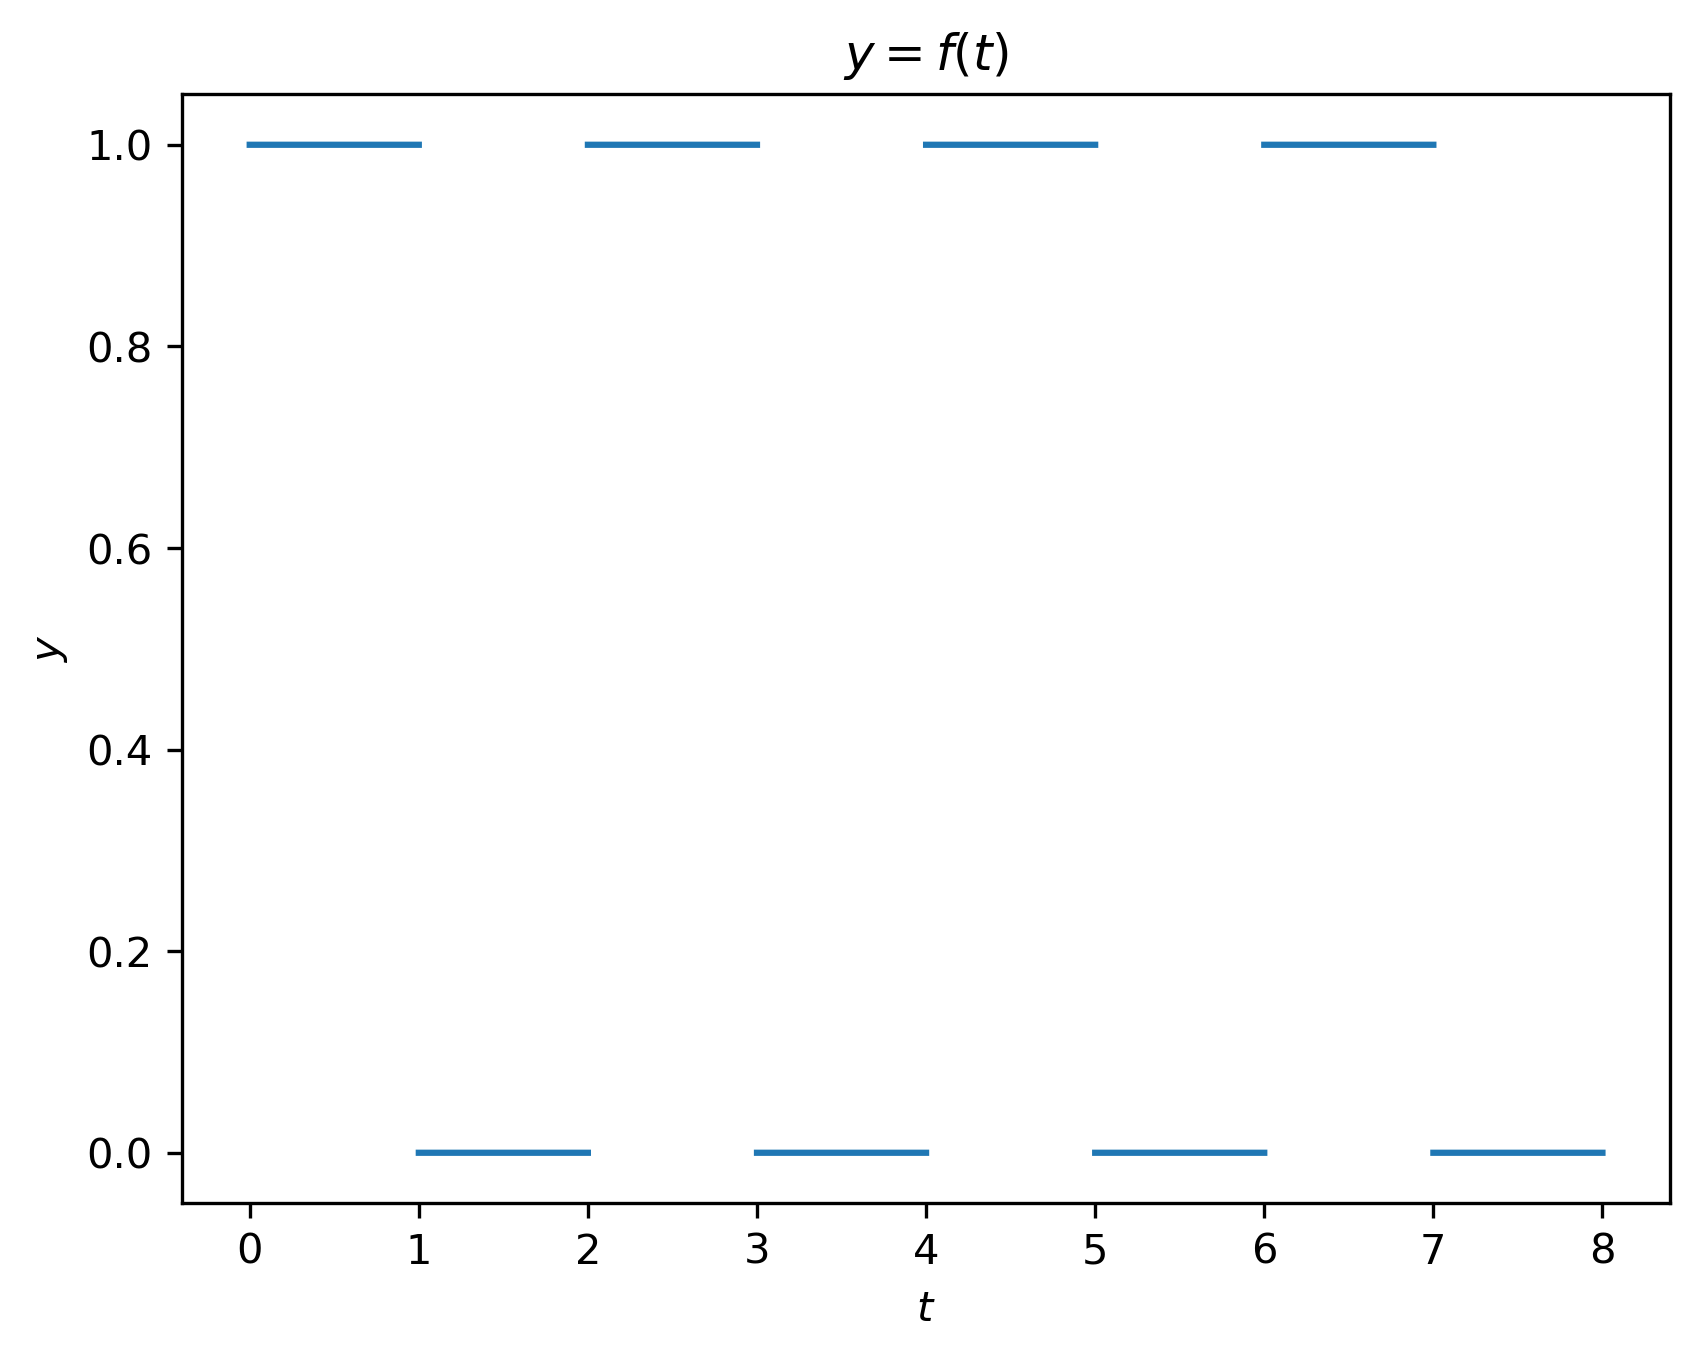
\includegraphics[scale=0.8]{plot step function.png}

    
\end{solution}



\part[2]\starscore34
Working directly from the definition,
explain why $F=\Laplace\Set{f}$ is given by
\[
F(s) = \frac{1}{s\lr(){1+e^{-s}}},\qquad s>0.
\]
\emph{Suggestion\/}:
Start by writing $F(s)$ as a series of simple integrals.


\begin{solution}
    We find that $f(t)$ is $0$ whenever $2n + 1 \leq t < 2n + 2$, so those integrals vanishes to $0$.

    So now, $F(s) = \int^{1}_{0} e^{-st} \mathrm dt + \int^{3}_{2} e^{-st} \mathrm dt + \int^{5}_{4} e^{-st} \mathrm dt + \int^{7}_{6} e^{-st} \mathrm dt + ...$

    Which means we can represent $F(s)$ by a series of relatively simple integrals like so:

    \[ F(s) = \sum^{\infty}_{k = 0} \int^{2k + 1}_{2k} e^{-st}\mathrm dt. \]

    Let us compute this antiderivative inside the sum.

    \[ \int^{2k + 1}_{2k} e^{-st} \mathrm dt = -\frac{1}{s} e^{-st} \Big|^{2k + 1}_{2k} = -\frac{1}{s}e^{-2sk - s} + \frac{1}{s}e^{-2sk} = \left ( \frac{1}{e^{2s}} \right)^k \left( \frac{1}{s} - \frac{1}{e^s s} \right). \]

    We can factor out the terms without the index of the sum outside of the sum.

    Additionally, $0 < \left( \frac{1}{e^{2s}} \right) < 1$ for any $s > 0$, which means we can apply the geometric series formula to it.

    So now we have:

    \[ F(s) = \left( \frac{1}{s} - \frac{1}{e^s s} \right) \sum^{\infty}_{k = 0} \left( \frac{1}{e^{2s}} \right)^k = \left( \frac{1}{s} - \frac{1}{e^s s} \right) \frac{1}{1 - \frac{1}{e^{2s}}}. \]

    Let us perform some algebraic manipulation:

    \begin{align*}
        \left( \frac{1}{s} - \frac{1}{e^s s} \right) \frac{1}{1 - \frac{1}{e^{2s}}}  &=  \left( \frac{1}{s} - \frac{1}{e^s s} \right) \frac{e^{2s}}{e^{2s} - 1} \\
                                                                                     &=  \left( \frac{1}{s} \right) \frac{e^{2s}}{(e^s + 1) (e^s - 1)} (1 - e^{-s}) \\
                                                                                     &=  \left( \frac{1}{s} \right) \frac{e^s}{(e^s + 1) (e^s - 1)} (e^s - 1) \\
                                                                                     &= \left( \frac{1}{s} \right) \frac{e^s}{e^s + 1} \\
                                                                                     &= \left( \left( \left( \frac{1}{s} \right) \frac{e^s}{e^s + 1} \right)^{-1} \right)^{-1} \\
                                                                                     &= \left( \frac{s(e^s + 1)}{e^s} \right)^{-1} \\
                                                                                     &= \left( s(1 + e^{-s}) \right)^{-1} \\
                                                                                     &= \frac{1}{s(1 + e^{-s})}
    \end{align*}

    As required.
\end{solution}

\end{parts}

\question\label{q:sinc}
The following improper integral is known to converge:
\[
I=\int_{-\infty}^\infty \frac{\sin(t)}{t}\,dt.
\]
(Note that the singularity at $t=0$ is removable,
because $\lim_{t\to 0}\frac{\sin(t)}t = 1$.)
\\
Find the exact value of $I$ by following the steps below:

\begin{parts}
\part[1]\starscore24
Find the Laplace Transform of $f(t) = \sin(t)$.
Call it $F(s)$; assume $s>0$.

\begin{solution}
    Let us apply the Laplace transform to $\sin(t)$.
    
    \begin{align*}
        \Laplace \Set{\sin(t)} = F(s) &= \int^{\infty}_{0} e^{-st} \sin(t) \mathrm dt \\
                                      &= \lim_{a \to \infty} \int^{a}_{0} e^{-st} \sin(t) \mathrm dt \\
        \intertext{Take $u = \sin(t)$, $\mathrm dv = e^{-st}$. Then $\mathrm du = \cos(t)$, and $v = -\frac{1}{s}e^{-st}$.}
                                      &= \lim_{a \to \infty} \left[ -\frac{\sin(t)}{s} e^{-st} \Big|^{a}_{0}  + \frac{1}{s}\int^{a}_{0} e^{-st}\cos(t) \mathrm dt \right]
        \intertext{Take $a = \cos(t)$, $\mathrm db = e^{-st}$. Then $\mathrm da = -\sin(t)$, and $b = -\frac{1}{s}e^{-st}$.}
                                      &= \lim_{a \to \infty} \left[ -\frac{\sin(t)}{s} e^{-st} \Big|^{a}_{0}  + \frac{1}{s}\left[
                                            -\frac{1}{s}e^{-st}\cos(t) \Big|^{a}_{0} - \frac{1}{s} \int^{a}_{0} e^{-st} \sin(t) \mathrm dt
                                      \right] \right] \\
        \intertext{Evaluating the first term, $-\frac{\sin(a)}{s}e^{-st} \to 0$ as $a \to \infty$, and $\sin(0) = 0$, which means the first term vanishes to zero.}
                                      &= \lim_{a \to \infty} \frac{1}{s}\left[
                                            -\frac{1}{s}e^{-st}\cos(t) \Big|^{a}_{0} - \frac{1}{s} \int^{a}_{0} e^{-st} \sin(t) \mathrm dt
                                      \right] \\
                                      &= \lim_{a \to \infty} -\frac{1}{s^2} e^{-st} \cos(t) \Big|^{a}_{0} - \frac{1}{s^2} \lim_{a \to \infty} \int^{a}_{0} e^{-st} \sin(t) \mathrm dt \\
                                      \intertext{We find that we can solve for $F(s)$, as it shows up again after integrating by parts.}
                                      &= \lim_{a \to \infty} -\frac{1}{s^2} e^{-st} \cos(t) \Big|^{a}_{0} - \frac{1}{s^2} F(s)
                                      \intertext{$-\frac{1}{s^2} e^{-st} \cos(t) \to 0$ as $a \to \infty$, and $-\frac{1}{s^2} e^{0} \cos(0) = -\frac{1}{s^2}$, so $\lim_{a \to \infty} -\frac{1}{s^2} e^{-st} \cos(t) \Big|^{a}_{0} = 0 - -\frac{1}{s^2} = \frac{1}{s^2}.$}
                                      &= \frac{1}{s^2} - \frac{1}{s^2} F(s)
    \end{align*}

    Now we have $F(s) = \frac{1}{s^2} - \frac{1}{s^2} F(s)$. Let us manipulate this equation to find $F(s)$ expressed as a rational function.

    \begin{align*}
        F(s) = \frac{1}{s^2} - \frac{1}{s^2} F(s) &\iff \left(1 + \frac{1}{s^2}\right)F(s) = \frac{1}{s^2} \\
                                                  &\iff F(s) = \frac{1}{s^2} \left( \frac{s^2 + 1}{s^2} \right)^{-1} \\
                                                  &\iff F(s) = \frac{1}{s^2 + 1}. \\
    \end{align*}

    So the Laplace transform of $\sin(x)$, defined by $F(s)$ is $\frac{1}{s^2 + 1}$.
\end{solution}


\begin{EnvUplevel}
Now, inspired by the form of $I$, we invent the function 
\[
G(s) = \int_0^\infty e^{-st}\lr(){\frac{\sin(t)}t}\,dt.
\]
This is the key step, with two essential properties:
\begin{enumerate}
\item When $s=0$, the factor $e^{-st}$ turns into $1$
and makes $G(0)$ very similar to the integral we seek;
and
\item the derivative of $G(s)$ has a simple form.
\end{enumerate}
\end{EnvUplevel}

\part[1]\starscore24
Express $G'(s)$ as a rational function of $s$ in the region where $s>0$.
\\
\emph{Suggestion\/}: Use without proof the natural extension of the
\href{https://en.wikipedia.org/wiki/Leibniz_integral_rule}{\emph{Leibniz integral rule}}
to this situation.

\begin{solution}
    Let us differentiate $G(s)$ and find a rational function of $s$ that expresses it.

    \begin{align*}
        G'(s) &= \frac{\mathrm d}{\mathrm ds} \int^{\infty}_{0} e^{-st} \left( \frac{\sin(t)}{t} \right) \mathrm dt \\
              &= \lim_{a \to \infty} \frac{\mathrm d}{\mathrm ds} \int^{a}_{0} e^{-st} \left( \frac{\sin(t)}{t} \right) \mathrm dt \\
              \intertext{Applying the Leibniz integral rule,}
              &= \lim_{a \to \infty} \int^{a}_{0} \frac{\partial}{\partial s} \left[ e^{-st} \left( \frac{\sin(t)}{t} \right) \right] \mathrm dt \\
              &= \lim_{a \to \infty} \int^{a}_{0} \frac{\sin(t)}{t} (-t) e^{-st} \mathrm dt \\
              &= \lim_{a \to \infty} -\int^{a}_{0} e^{-st}\sin(t) \mathrm dt \\
              &= -\lim_{a \to \infty} \int^{a}_{0} e^{-st}\sin(t) \mathrm dt \\
              \intertext{Using our results from the previous question,}
              &= -\frac{1}{s^2 + 1}
    \end{align*}
\end{solution}



\part[1]\starscore14
Use the result above to find $\lim_{R\to\infty}\lr[]{G(R)-G(0)}$.

\begin{solution}
    By FTC2, $G(R) - G(0) = \int^{R}_{0} G'(u) \mathrm du$.

    Therefore,

    \[ \int^{R}_{0} G'(u) \mathrm du = \int^{R}_{0} -\frac{1}{u^2 + 1} \mathrm du = -\arctan{R} + \arctan{0}. \]

    So $\lim_{R \to \infty} \left[ G(R) - G(0) \right] = \lim_{R \to \infty} -\arctan{R} + \arctan{0} = -\frac{\pi}{2}$.
\end{solution}


\part[1]\starscore14
Determine the exact value of $I$.

\begin{solution}
    Let us first show that $f(t) = \frac{\sin(t)}{t}$ is even. A real valued function $f$ is even if $f(-x) = f(x)$.
    \begin{proof}
        Consider $f(-t) = \frac{\sin(-t)}{-t}$. Then $\frac{\sin(-t)}{-t} = -\frac{\sin(t)}{-t} = \frac{\sin(t)}{t} = f(t)$. Clearly $f(t)$ is even.
    \end{proof}

    As it is even,  $\int^\infty_{-\infty} \frac{\sin(t)}{t} \mathrm dt = 2 \int^{\infty}_{0} \frac{\sin(t)}{t} \mathrm dt = 2G(0)$.

    Time to find out the value of $G(0)$. First let us determine the value of $\lim_{R \to \infty} G(R)$, and we can work with the value of the limit to find $G(0)$.

    As $R \to \infty$, $\int^\infty_{0} e^{-Rt} \frac{\sin(t)}{t} \mathrm dt \to 0$ as $e^{-st}$ decreases faster than any trigonometric function.
    
    Therefore $\lim_{R \to \infty} G(R) = 0$. Recall $\lim_{R \to \infty} \left[ G(R) - G(0) \right] = -\frac{\pi}{2}$. 
    
    So it must follow that $\lim_{R \to \infty} \left[ G(R) - G(0) \right] = -\frac{\pi}{2} \iff 0 - G(0) = \frac{-\pi}{2} \iff G(0) = \frac{\pi}{2}$.

    Therefore, $\int^{\infty}_{-\infty} = 2G(0) = \pi$.
\end{solution}


\end{parts}


\vskip 0pt plus 10fill
\clearpage

\end{questions}  %%%%%%%%%%%%%%%%%%%%%%%%%%%%%%%%%%%%%%%


\bigbreak\hrule\medskip

\noindent{\textbf{Notes and Comments}}

\noindent
The Fourier theory is used throughout applied mathematics,
from the theory of waves, heat flow, and probability, to
quantum mechanics.

The idea used in Question~\ref{q:shanks}
to accelerate convergence of partial
sums of a given series can be applied to any
convergent sequence.
It is known as 
\href{https://en.wikipedia.org/wiki/Shanks_transformation}{\emph{the Shanks Transformation}},
in spite of having been invented and published
decades before Daniel Shanks's paper of 1955.
It is one of a large number of methods for
accurately predicting the limit of a slowly-converging
sequence.
(To learn more about such methods, see, e.g.,
Weniger, E. J., 
\emph{Nonlinear sequence transformations for the
acceleration of convergence and the
summation of divergent series,}
\url{https://arxiv.org/pdf/math/0306302.pdf}.)

The idea in Question~\ref{q:sinc} is popularly known
as Feynman's Integral Trick: 
it has many fascinating applications.
There are nice discussions online at 
\href{https://www.cantorsparadise.org/richard-feynmans-integral-trick-e7afae85e25c/}{\emph{Cantor's Paradise}} and 
\href{https://zackyzz.github.io/feynman.html}{\emph{a personal site of Zaharia Burghelea}}.
The function $\sin(t)/t$ (extended with the value $1$ when $t=0$) comes up
often enough to deserve a special name: it's known as the \href{https://en.wikipedia.org/wiki/Sinc_function}{\emph{sinc function}}.


\end{document}
